\documentclass[conference]{IEEEtran}
\IEEEoverridecommandlockouts
% The preceding line is only needed to identify funding in the first footnote. If that is unneeded, please comment it out.
\usepackage{cite}
\usepackage{amsmath,amssymb,amsfonts}
\usepackage{graphicx}
\usepackage{textcomp}
\usepackage{hyperref}
\usepackage{url}
\usepackage{xcolor}
\usepackage{subcaption}
\def\BibTeX{{\rm B\kern-.05em{\sc i\kern-.025em b}\kern-.08em
    T\kern-.1667em\lower.7ex\hbox{E}\kern-.125emX}}
\begin{document}

\title{\emph{NautDB}: Towards a Hybrid Runtime for Processing Compiled Queries
\thanks{This work was supported by NSF Award \#1640864. Opinions, findings and conclusions expressed in this material are those of the authors and do not necessarily reflect the views of the National Science Foundation.}
}

\author{\IEEEauthorblockN{Samuel Grayson}
\IEEEauthorblockA{\textit{Department of Computer Science} \\
\textit{University of Texas at Dallas}\\
samuel.grayson@utdallas.edu}
% \and
% \IEEEauthorblockN{Kyle Hale}
% \IEEEauthorblockA{\textit{Department of Computer Science} \\
% \textit{Illinois Institute of Technology}\\
% khale@cs.iit.edu}
% \and
% \IEEEauthorblockN{Boris Glavic}
% \IEEEauthorblockA{\textit{Department of Computer Science} \\
% \textit{Illinois Institute of Technology}\\
% bglavic@iit.edu}
}

\newcommand{\todo}[1]{\textcolor{red}{#1}}

\maketitle

\begin{abstract}
General purpose operating and database system suffer under the load of their generality which makes achieving optimal performance extremely hard, especially on modern hardware.
The goal of this research is to integrate specialization techniques from the OS community (hybrid runtimes) and DB community (compiled queries) for high-performance query processing on modern hardware. We envision a system called \emph{NautDB}, a hybrid dataflow runtime for executing compiled queries. As a first step towards our goal we evaluate the performance of compiled queries on Linux and run as a \emph{Nautilus} hybrid runtime using a simple prototype.
Our results demonstrate that combining these specialization techniques has transformative potential for building the next generation (distributed) high-performance query processing systems and big data platforms.
\end{abstract}

\begin{IEEEkeywords}
hybrid runtimes, light-weight kernels, compiled query processing, high-performance query processing
\end{IEEEkeywords}

%%%%%%%%%%%%%%%%%%%%%%%%%%%%%%%%%%%%%%%%
\section{Introduction}

  Both the operating system (OS) and database (DB) communities have strived to build general purpose systems which exhibit reasonable performance for a wide variety of applications and are user friendly.
  %
  However, the performance of general purpose operating and database systems suffers~\cite{GICEVA:2016:OS_SUPPORT} from being overly generic and hiding implementation details behind multiple layers of abstraction.
  %
Both communities have worked on achieving better performance on modern hardware without sacrificing ease of use. Specifically, OS researchers have introduced hybrid runtimes~\cite{HALE:2017:MULTIVERSE,HALE:2016:MULTIVERSE,HALE:2015:NAUTILUS,HALE:2016:HRTHVM} as a means to give an application more immediate access to hardware and control over OS behavior while database researchers have studied query compilation to specialize a database execution engine to a particular query~\cite{SK16,N11}.

The ultimate goal of this research is to integrate, for the first time, these specialization techniques from the OS community (hybrid runtimes) and DB community (compiled queries) for high-performance query processing.
  %
As a first step towards this goal, we build a testing prototype that uses hand-optimized query operator implementations and use this prototype to evaluate the potential performance benefit of running compiled queries as a hybrid runtime.
%
Our preliminary results demonstrate that, even though this first version of our prototype is still quite naive, we can achieve better and more predictable performance through specialization.
%


% %%%%%%%%%%%%%%%%%%%%%%%%%%%%%%%%%%%%%%%%
% \section{Related Work}



%%%%%%%%%%%%%%%%%%%%%%%%%%%%%%%%%%%%%%%%
\section{Preliminary Evaluation}

As a preliminary assessment of the potential of our idea we have built an initial testing prototype which consists of manually optimized implementations of common database query operators. We then evaluate the performance of this prototype on a standard Linux distribution and as a hybrid runtime embedded into the Nautilus aerokernel. The purpose of this experiment is to evaluate how the highly specialized implementation of OS functionality like, e.g., memory management, and the more immediate control over OS features provided by hybrid runtimes benefit evaluation of compiled, high-performance query plans (like the ones already produced by modern query compilers used in main memory database systems~\cite{N11}). 

%%%%%%%%%%%%%%%%%%%%%%%%%%%%%%%%%%%%%%%%
\subsection{Testing Prototype}
\label{sec:testing-prototype}

We have implemented the prototype in C. It supports several important database operators including selection, projection, and sort.  Here we focus on the implementation of the sort operator, because this  operator is of essential importance in database systems to implement operators like aggregation and joins (merge-join). Our implementation sorts an input table that is stored as columnar chunks. That is each column of the table is stored separately as a collections of large arrays that we coin chunks in this work. Our sort implementation uses counting sort to sort the data within a chunk and merged sort to sort across chunks. We have implemented a row-oriented and a column-oriented variant of this sort algorithm.

%%%%%%%%%%%%%%%%%%%%%%%%%%%%%%%%%%%%%%%%
\subsection{Experimental Setup}
\label{sec:experimental-setup}

We ran our prototype on Linux (linux kernel 4.17.6) and as hybrid runtime using Nautilus\footnote{\url{https://github.com/HExSA-Lab/nautilus} - git commit \texttt{2fb4e52816}}~\cite{HALE:2015:NAUTILUS,HALE:2016:HRTHVM}. 
All experiments were run on a 16-core x86\_64 AMD EPYC machine with 4 NUMA nodes.
We sort a table consisting of  $256$ chunks varying the number of elements per chunk and the number of columns in the table.

%%%%%%%%%%%%%%%%%%%%%%%%%%%%%%%%%%%%%%%%
\subsection{Experimental Results}
\label{sec:experimental-results}



%%%%%%%%%%%%%%%%%%%%%%%%%%%%%%%%%%%%%%%%
\begin{figure*}[t]
  \centering
  \begin{minipage}{0.32\linewidth}
    \centering
    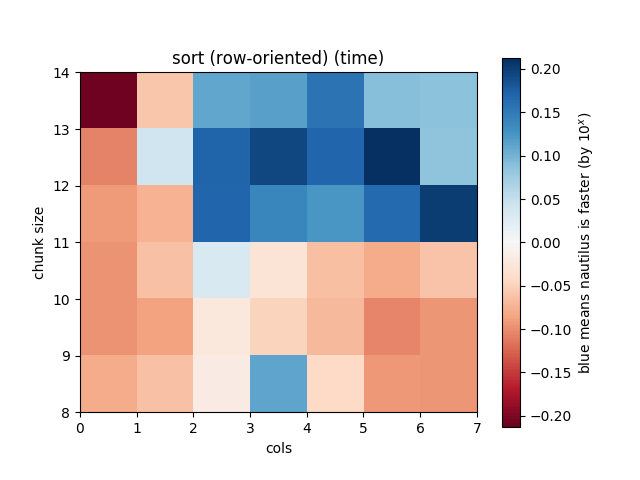
\includegraphics[width=1\linewidth]{../plots/sort_2d.png}
    \subcaption{Row-oriented sorting for a $128$ column table with 256 chunks}\label{fig:sort2d}
  \end{minipage}
  \begin{minipage}{0.32\linewidth}
    \centering
  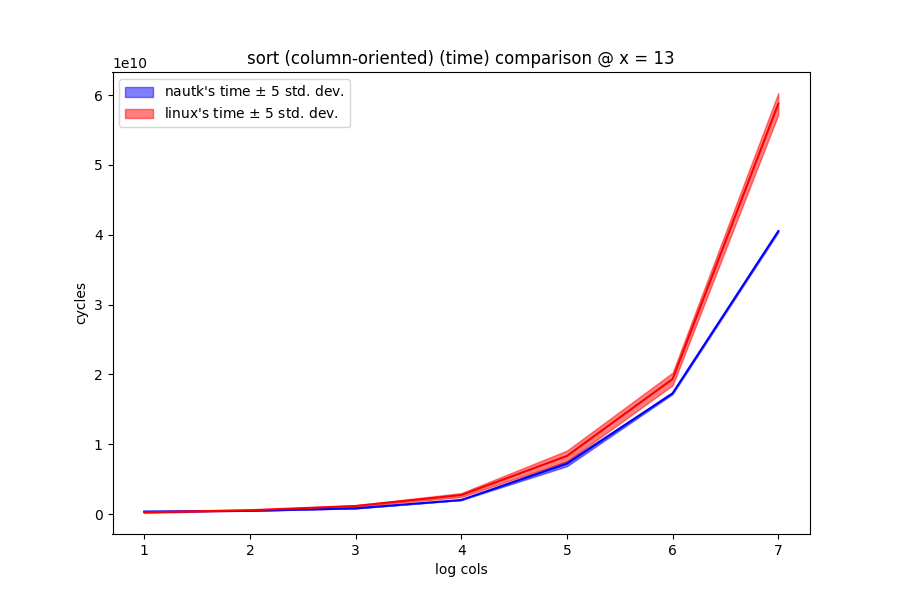
\includegraphics[width=1\linewidth]{../plots/sort.png}
    \subcaption{Column-oriented sort measuring runtime and uncertainty (\todo{2 standard deviations?}) for a fixed chunk size \todo{WHICH ONE}, varying the number of columns}\label{fig:colsort}
  \end{minipage}
  \begin{minipage}{0.32\linewidth}
    \centering
      \begin{tabular}{l || r | r }
        \textbf{Kernel}    & TLB misses  & Instruction cache misses \\
        \hline\hline
        \textbf{Linux}     & 135,000,000 & 3,030,000 \\
         \textbf{Nautilus} &           1 &   480,000 \\
      \end{tabular}

    \subcaption{TLB and cache misses for row-oriented sorting of a $128$ column table with $8192$ elements per chunk}\label{fig:cache_miss}
  \end{minipage}

\caption{Evaluating the performance of sort on Nautilus and Linux.}
  \label{fig:perf-eval}
\end{figure*}
%%%%%%%%%%%%%%%%%%%%%%%%%%%%%%%%%%%%%%%%

The results of these experiments are shown in Figure~\ref{fig:perf-eval}.   For larger number of columns and larger chunks, Nautilus outperforms Linux. This is because Nautilus has larger page size and incurs less TLB misses (see Table \ref{fig:cache_miss}).   Furthermore, we see (Figure~\ref{fig:colsort}) that Nautilus performance if much more predictable than Linux. This effect is observed even in configurations where Linux outperforms Nautilus. The main reason for this is that Nautilus does not have scheduling interrupts, so it avoids unpredictable detours which also leads to better cache performance.



%%%%%%%%%%%%%%%%%%%%%%%%%%%%%%%%%%%%%%%%
\subsection{Discussion}
\label{sec:discussion}


These preliminary result demonstrate that specialization allows us to tune the OS and DB ending for a query workload and that compiled queries that consist of highly-specialized code benefit from a hybrid runtime environment.
Furthermore, hybrid runtimes have much more predictable performance than general purpose OS which will benefit performance for parallelization of our prototype (e.g., using the bulk-synchronous model).
While our prototype based on the \emph{Nautilus} aerokernel does not outperform Linux on all parameter settings, it consistently shows better TLB and instruction cache behavior as well as more consistent performance (predictability). This is even though the  research prototype implementation of OS features in Nautilus has to compete with a mature industrial strength implementation in Linux that has been optimized by a horde of skilled developers over decades. 

%%%%%%%%%%%%%%%%%%%%%%%%%%%%%%%%%%%%%%%%
\section{Our Vision for NautDB}
\label{sec:our-vision-nautdb}

As a long term goal, we envision \emph{NautDB}, a hybrid dataflow runtime which executes tasks that are represented as compiled (machine) code. The frontend of NautDB will be a query compiler that translates high-level queries (SQL or another declarative and high-level language) into compiled low-level tasks to be executed by the dataflow runtime. The present paper represents the first step towards this goal.


%%%%%%%%%%%%%%%%%%%%%%%%%%%%%%%%%%%%%%%%
\section{Conclusions and Future Work}
\label{sec:concl-future-work}

This work demonstrated the potential of combining hybrid runtimes with compiled query processing. In future work, I plan to evaluate additional database operators, parallel execution of such operators, and evaluate effect of context switches and interrupts that can be controlled in Nautilus, but not in Linux. 

%%%%%%%%%%%%%%%%%%%%%%%%%%%%%%%%%%%%%%%%
  \bibliographystyle{abbrv}
  \bibliography{../kyle,../sam,../boris}


\end{document}

%%% Local Variables:
%%% mode: latex
%%% TeX-master: t
%%% End:
